\documentclass[a4paper,11pt,fleqn]{jarticle}
\usepackage[dvipdfmx]{graphicx}
\usepackage{float}
\usepackage{amsmath}
\usepackage{fancyhdr}

\def \vec#1{\mbox{\boldmath $#1$}} %ベクトルマクロ
\def \bun#1#2{\left(\frac{#1}{#2}\right)} %括弧つき分数マクロ
\def \rot{\nabla \times} %rot
\def \div{\nabla \cdot} %div
\def \intt{\int\!\!\!\int} %2重積分
\def \inttt{\int\!\!\!\int\!\!\!\int} %3重積分

% ページレイアウト
\setlength{\topmargin}{10mm}
  \addtolength{\topmargin}{-1in}
\setlength{\oddsidemargin}{30mm}
  \addtolength{\oddsidemargin}{-1in}
\setlength{\textwidth}{150mm}
\setlength{\textheight}{250mm}
\setlength{\headsep}{2zw}
\setlength{\headheight}{2zw}
\setlength{\topskip}{15mm}
\linespread{1.0}

% サブセクションを1.,2.にする設定
\renewcommand{\thesubsection}{\arabic{subsection}.}

% サブサブセクションを(1),(2)にする設定
\renewcommand{\thesubsubsection}{(\arabic{subsubsection})}

% 大問2の3番目の計算式のラベルを(2.3)にする設定
% 計算式の参照には\eqref{eq:hoge}を使う
\makeatletter
  \renewcommand{\theequation}{\arabic{subsection}.\arabic{equation}}
  \@addtoreset{equation}{subsection}
\pagestyle{fancy}
% ヘッダーの設定
  \lhead[物理数学 2016.04.14]{\leftmark}
  \rhead[\leftmark]{物理数学 2016.04.14}
\renewcommand{\headrulewidth}{0pt}
\makeatother


\begin{document}


\begin{center}
\begin{Large}
演習問題その4 ベクトル解析(4)
\end{Large}
\end{center}

物理でよく使われる座標系には、デカルト座標系(カルテシアン座標系、直交座標系)以外にも円柱座標系、極座標系(球座標系)などがある(図1)。
\begin{figure*}[htbp]
\begin{center}
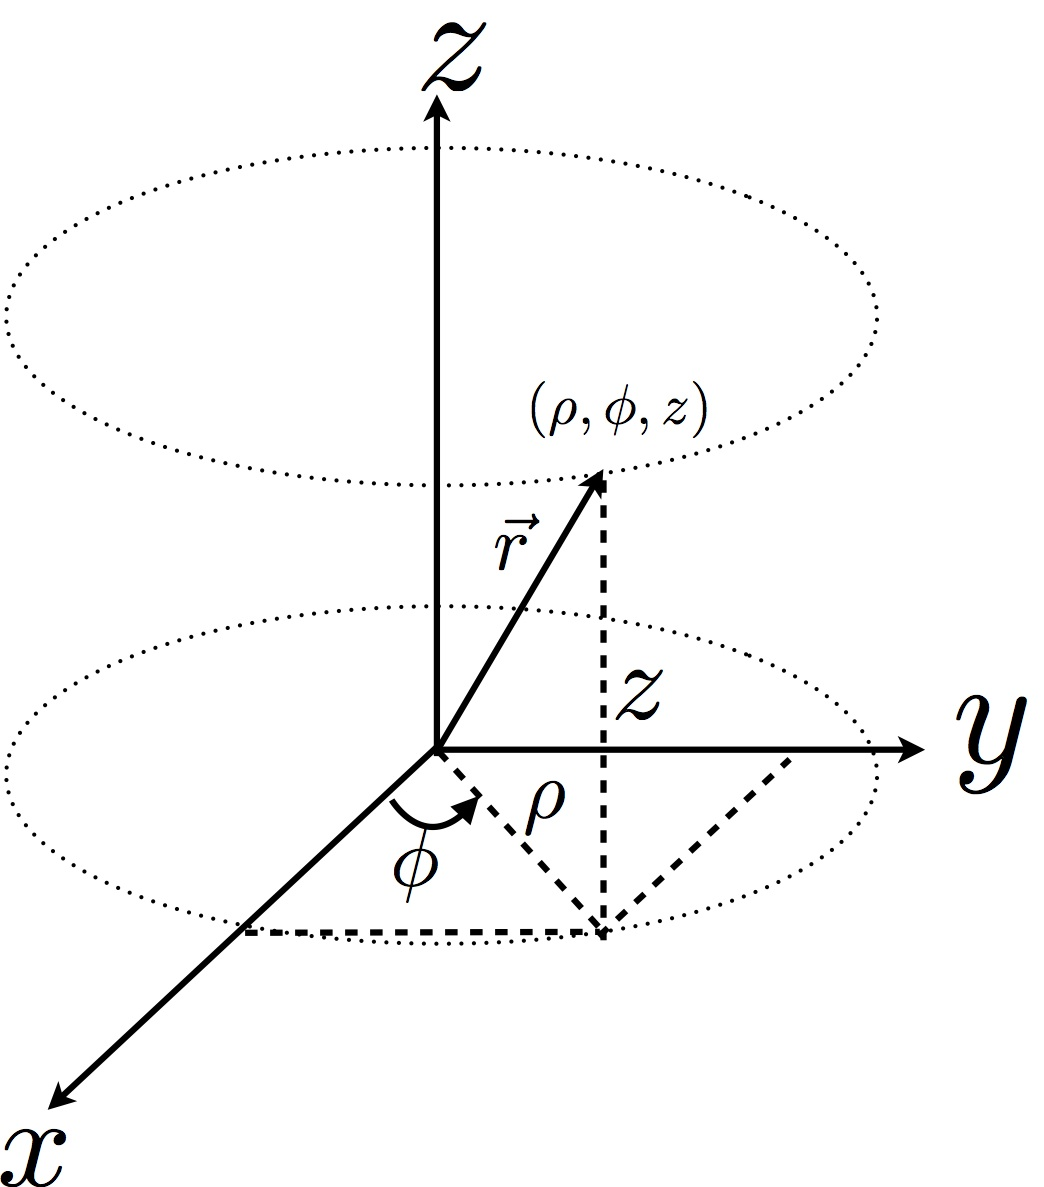
\includegraphics[height=7cm,keepaspectratio]{5fig/cylinder.eps}
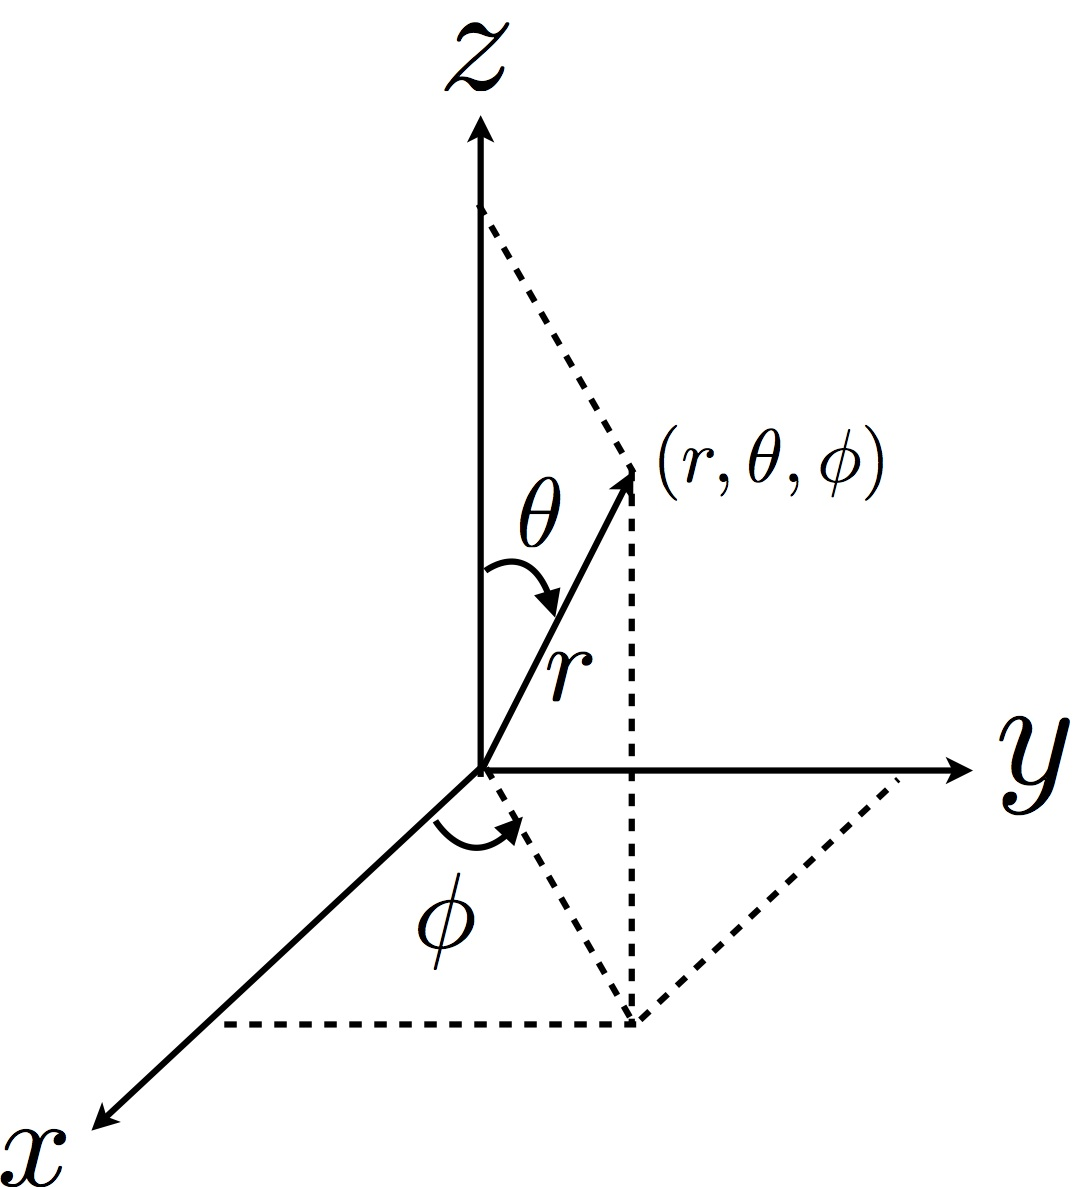
\includegraphics[height=7cm,keepaspectratio]{5fig/polar.eps}
\caption{左: 円筒座標系 右:極座標系 }
\label{fig:tmt6}
\end{center}
\end{figure*}
\subsection{}
デカルト座標系$(x,y,z)$と円柱座標系$(\rho ,\phi ,z)$の間の座標変換を考える。
\subsubsection{$(x,y,z)を(\rho ,\phi ,z)を用いて表せ。また、(\rho ,\phi ,z)を(x,y,z)を用いて表せ。$}
\subsubsection{$\vec{e}_{\rho},\vec{e}_{\phi},\vec{e}_zを\vec{e}_x,\vec{e}_y,\vec{e}_zを用いて表せ。また、\vec{e}_x,\vec{e}_y,\vec{e}_zを\vec{e}_{\rho},\vec{e}_{\phi},\vec{e}_zを用いて表せ。$}


\newpage
\subsubsection{$デカルト座標系で、\vec{A}=z\vec{e}_x-2x\vec{e}_y+y\vec{e}_zと表されるベクトル\vec{A}を円柱座標系で表せ。$}

\vspace{80mm}
\subsection{}
デカルト座標系$(x,y,z)$と極座標系$(r ,\theta ,\phi)$の間の座標変換を考える。
\subsubsection{$(x,y,z)を(r ,\theta ,\phi )を用いて表せ。また、(r ,\theta ,\phi )を(x,y,z)を用いて表せ。$}
\subsubsection{$\vec{e}_{r},\vec{e}_{\theta},\vec{e}_{\phi}を\vec{e}_x,\vec{e}_y,\vec{e}_zを用いて表せ。また、\vec{e}_x,\vec{e}_y,\vec{e}_zを\vec{e}_{r},\vec{e}_{\theta},\vec{e}_{\phi}を用いて表せ。$}

\newpage
\subsubsection{$極座標系で、\vec{A}=r^2\sin\theta\vec{e}_{\theta}と表されるベクトル\vec{A}をデカルト座標で表せ。$}

\vspace{90mm}
\subsection{}
$f=x+2y+z$とする。極座標系での$\nabla f$をそれぞれ求めよ。

\newpage
\subsection{}
円柱座標系$(\rho ,\phi ,z)$で$\vec{a}=\rho\cos\phi\vec{e}_{\rho}-z\sin\phi\vec{e}_{\phi}+\rho z\vec{e}_z$と表されるベクトル$\vec{a}$について、$\nabla\cdot\vec{a},~\nabla\times\vec{a}$をそれぞれ求めよ。

\newpage
\subsection{}
円柱座標系$(\vec{e}_{\rho},\vec{e}_{\phi},\vec{e}_z)$について、以下の問いに答えよ。
\subsubsection{}
基底ベクトルの時間微分が$\frac{d}{d t}\vec{e}_{\rho}=\dot{\phi}\vec{e}_{\phi},~\frac{d}{d t}\vec{e}_{\phi}=-\dot{\phi}\vec{e}_{\rho}$であることを示せ。

\vspace{80mm}
\subsubsection{}
質点の速度$\vec{v}$、加速度$\vec{a}$を円筒座標系で表せ。

\newpage
\subsection{}
以下の問いに答えよ。
\subsubsection{$\vec{a}=(3x^2+y^2)\vec{e}_x+2xy\vec{e}_y+z^2\vec{e}_zであるとき、x=\rho\cos\phi ,~y=\rho\sin\phi ,~z=zとして次式を媒介変数\rho ,\phi ,zで表せ(\vec{a}やd\vec{r}を円柱座標系の基底ベクトルを用いて表す必要はない)$}

\begin{center}
$\int_C \vec{a}\cdot d\vec{r}$
\end{center}

\vspace{80mm}
\subsubsection{$z=0上の平面において、Cが半径3の半円の弧を描くとき(1)の線積分の値を求めよ(つまり、Cは\rho =3=一定,\phi :[0\rightarrow\pi ]となる)$}

\newpage
\subsection{}
$\vec{b}=-z\vec{e}_{x}-3x^2y\vec{e}_{y}+2x^2y^2\vec{e}_{z}$とする.図のような立方体の面EFGHを除く5つの面を$S$とし,閉曲線E→H→G→F→Eを$C$とするとき,$\int_S (\nabla\times \vec{b})\cdot \mathrm{d}\vec{S}$と$\int_C \vec{b} \cdot \mathrm{d}\vec r$を計算することにより,ストークスの定理が成り立っていることを確かめよ.
\begin{center}
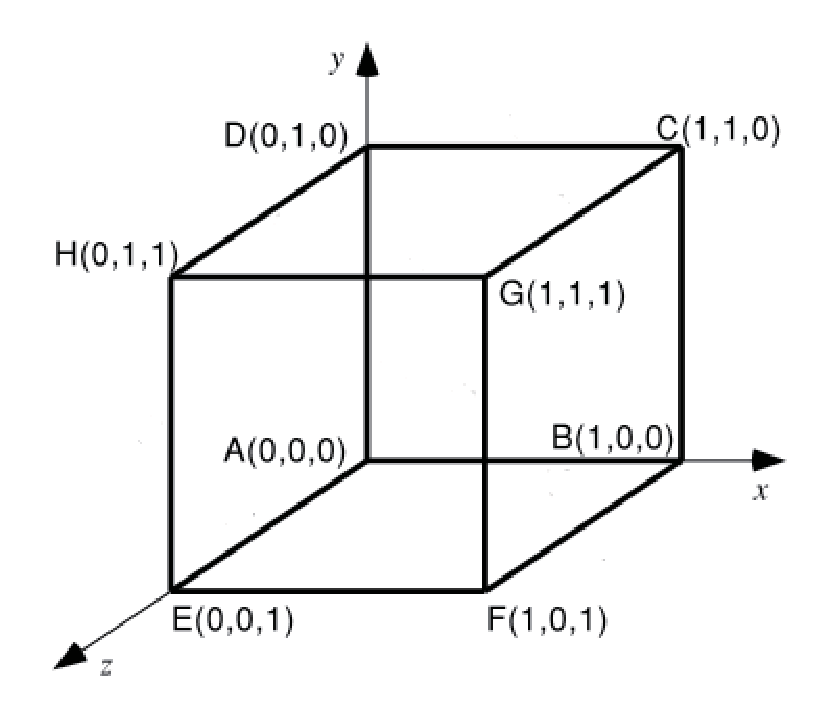
\includegraphics[width=.4\textwidth,bb=19 19 400 340]{5fig/rippou.eps}
\label{rippou}
\end{center}

\newpage
\subsection{}
放物面$z=1-(x^2+y^2)$のうち,$z\ge 0$の領域を$S$とする.
$\vec{a}=-2y \vec{e}_{x}+ x \vec{e}_{y}+ z \vec{e}_{z}$とするとき,$\int_S(\nabla\times \vec{a})\cdot \mathrm{d}\vec{S}$を計算せよ.ただし,$d\vec{S}$の向きは$+z$方向とする。\\
(ヒント:面積分しない)


\vspace{90mm}
\subsection{}
ある場から物体に働く力$\vec{F}$が、スカラー場$\phi$を用いて$\vec{F}=-\nabla\phi$と書けるとき、この力$\vec{F}$が保存力であることを示せ。ただし、保存力とは、任意の2点間を移動するときになされる仕事が経路に依らないような力のことである。\\
(ヒント:任意のスカラー場$\phi$に対して$\nabla\times (\nabla\phi )$をとると...?)

\newpage
\subsection{$+\alpha$問題}
任意の直交曲線座標系(円柱座標系や球座標系など)$q_1,q_2,q_3$における$\nabla{f}$の表記が以下の通りであることを示したい。
\begin{eqnarray*}
\nabla{f}=\frac{\partial{f}}{h_1\partial{q_1}}\vec{e}_1+\frac{\partial{f}}{h_2\partial{q_2}}\vec{e}_2+\frac{\partial{f}}{h_3\partial{q_3}}\vec{e}_3
\end{eqnarray*}
ただし、$\delta{\vec{r}}=\delta{x}\vec{e}_x+\delta{y}\vec{e}_y+\delta{z}\vec{e}_z=h_1\delta{q_1}\vec{e}_1+h_2\delta{q_2}\vec{e}_2+h_3\delta{q_3}\vec{e}_3$である。
\subsubsection{$まずデカルト座標系において(x,y,z)\rightarrow(x+\delta{x},y+\delta{y},z+\delta{z})となったときのfの変化量\delta fを求めることにより、\nabla f\cdot\delta\vec{r}となることを示せ。$}

\vspace{80mm}
\subsubsection{$次に任意の直交曲線座標系で(q_1,q_2,q_3)\rightarrow(q_1+\delta{q_1},q_2+\delta{q_2},q_3+\delta{q_3})となったときのfの変化量\delta fを求め、題意を示せ。$}

\newpage
\subsubsection{$上記の結果を用いて、極座標系における\nabla fを求めよ。$}
補足:$h_i(i=1,2,3)$について、
\begin{eqnarray*}
h_i\delta{q}_i\vec{e}_i=\frac{\partial{x}}{\partial{q_i}}\delta{q}_i\vec{e}_x+\frac{\partial{y}}{\partial{q_i}}\delta{q}_i\vec{e}_y
+\frac{\partial{z}}{\partial{q_i}}\delta{q}_i\vec{e}_z
\end{eqnarray*}
となるので$h_i$は以下のように表せる:
\begin{eqnarray*}
h_i=\sqrt{\left(\frac{\partial{x}}{\partial{q_i}}\right)^2+\left(\frac{\partial{y}}{\partial{q_i}}\right)^2+\left(\frac{\partial{z}}{\partial{q_i}}\right)^2}
\end{eqnarray*}

\newpage
\subsubsection{時間が余った人向け}
(3)で求めた、極座標についての$\nabla$を用いて$\Delta f$が以下のように記述できることを示せ。
\begin{eqnarray*}
\Delta f=\frac{1}{r^2}\frac{\partial}{\partial r}\left(r^2\frac{\partial f}{\partial r}\right)+\frac{1}{r^2\sin\theta}\frac{\partial}{\partial \theta}\left(\sin\theta\frac{\partial f}{\partial \theta}\right)+\frac{1}{r^2{\sin}^2\theta}\frac{{\partial}^2 f}{\partial {\phi}^2}
\end{eqnarray*}
補足:\\
$\Delta f=\nabla\cdot (\nabla f).~$極座標の単位ベクトルの座標微分($\frac{\partial}{\partial \phi}\vec{e}_{\theta}$など)はゼロでないことに注意。


\end{document}